% Create a Table of Contents in Beamer
\documentclass[10pt,t]{beamer}
% Theme choice:
\usetheme{Singapore}
\usecolortheme{whale}
\setbeamercolor{titlelike}{fg=blue,bg=white}
\setbeamercolor{frametitle}{fg=blue,bg=white}
\setbeamertemplate{frametitle}[default][left]
\setbeamertemplate{navigation symbols}{}

\usepackage{graphicx}
\usepackage{amsmath}
\usepackage{amsfonts}
\usepackage{amssymb}
\usepackage{amsthm}
\usepackage{ulem}

% Title page details: 
\title{Chapter 1: Linear Regression} 
\author{Taylor Okonek \& Charlie Wolock}
\date{\today}


\begin{document}
	% Title page frame
	\begin{frame}
	\titlepage 
\end{frame}

\begin{frame}{Learning objectives}
By the end of Chapter 1, you should be able to:
\begin{itemize}
	\item Formulate a regression model, given a scientific or statistical question
	\item Interpret the coefficients for a (simple or multiple) linear regression model
	\item Interpret confidence intervals and p-values for linear regression coefficients
	\item Classify variables according to their role in a linear regression model (e.g., outcome, predictor, potential confounder, effect modifier, precision variable)
	\item Use \texttt{R} to fit a linear regression model (and know where in the output to look for the information we need to interpret results)
	\item Create graphs to support your linear regression analysis
\end{itemize}
\end{frame}

% Outline frame
\begin{frame}{Outline}
\tableofcontents
\end{frame}

\AtBeginSection[ ]
{
\begin{frame}{Outline}
\tableofcontents[currentsection]
\end{frame}
}

% Presentation structure
\section{Simple Linear Regression}

\begin{frame}{Simple linear regression}

We collect 150 leaves, and record their lengths and widths in inches. We hypothesize that leaves with larger lengths will also tend to have larger widths. To represent this graphically, we plot all of the data below\dots

\vspace{0.3cm}

\begin{figure}
	\centering 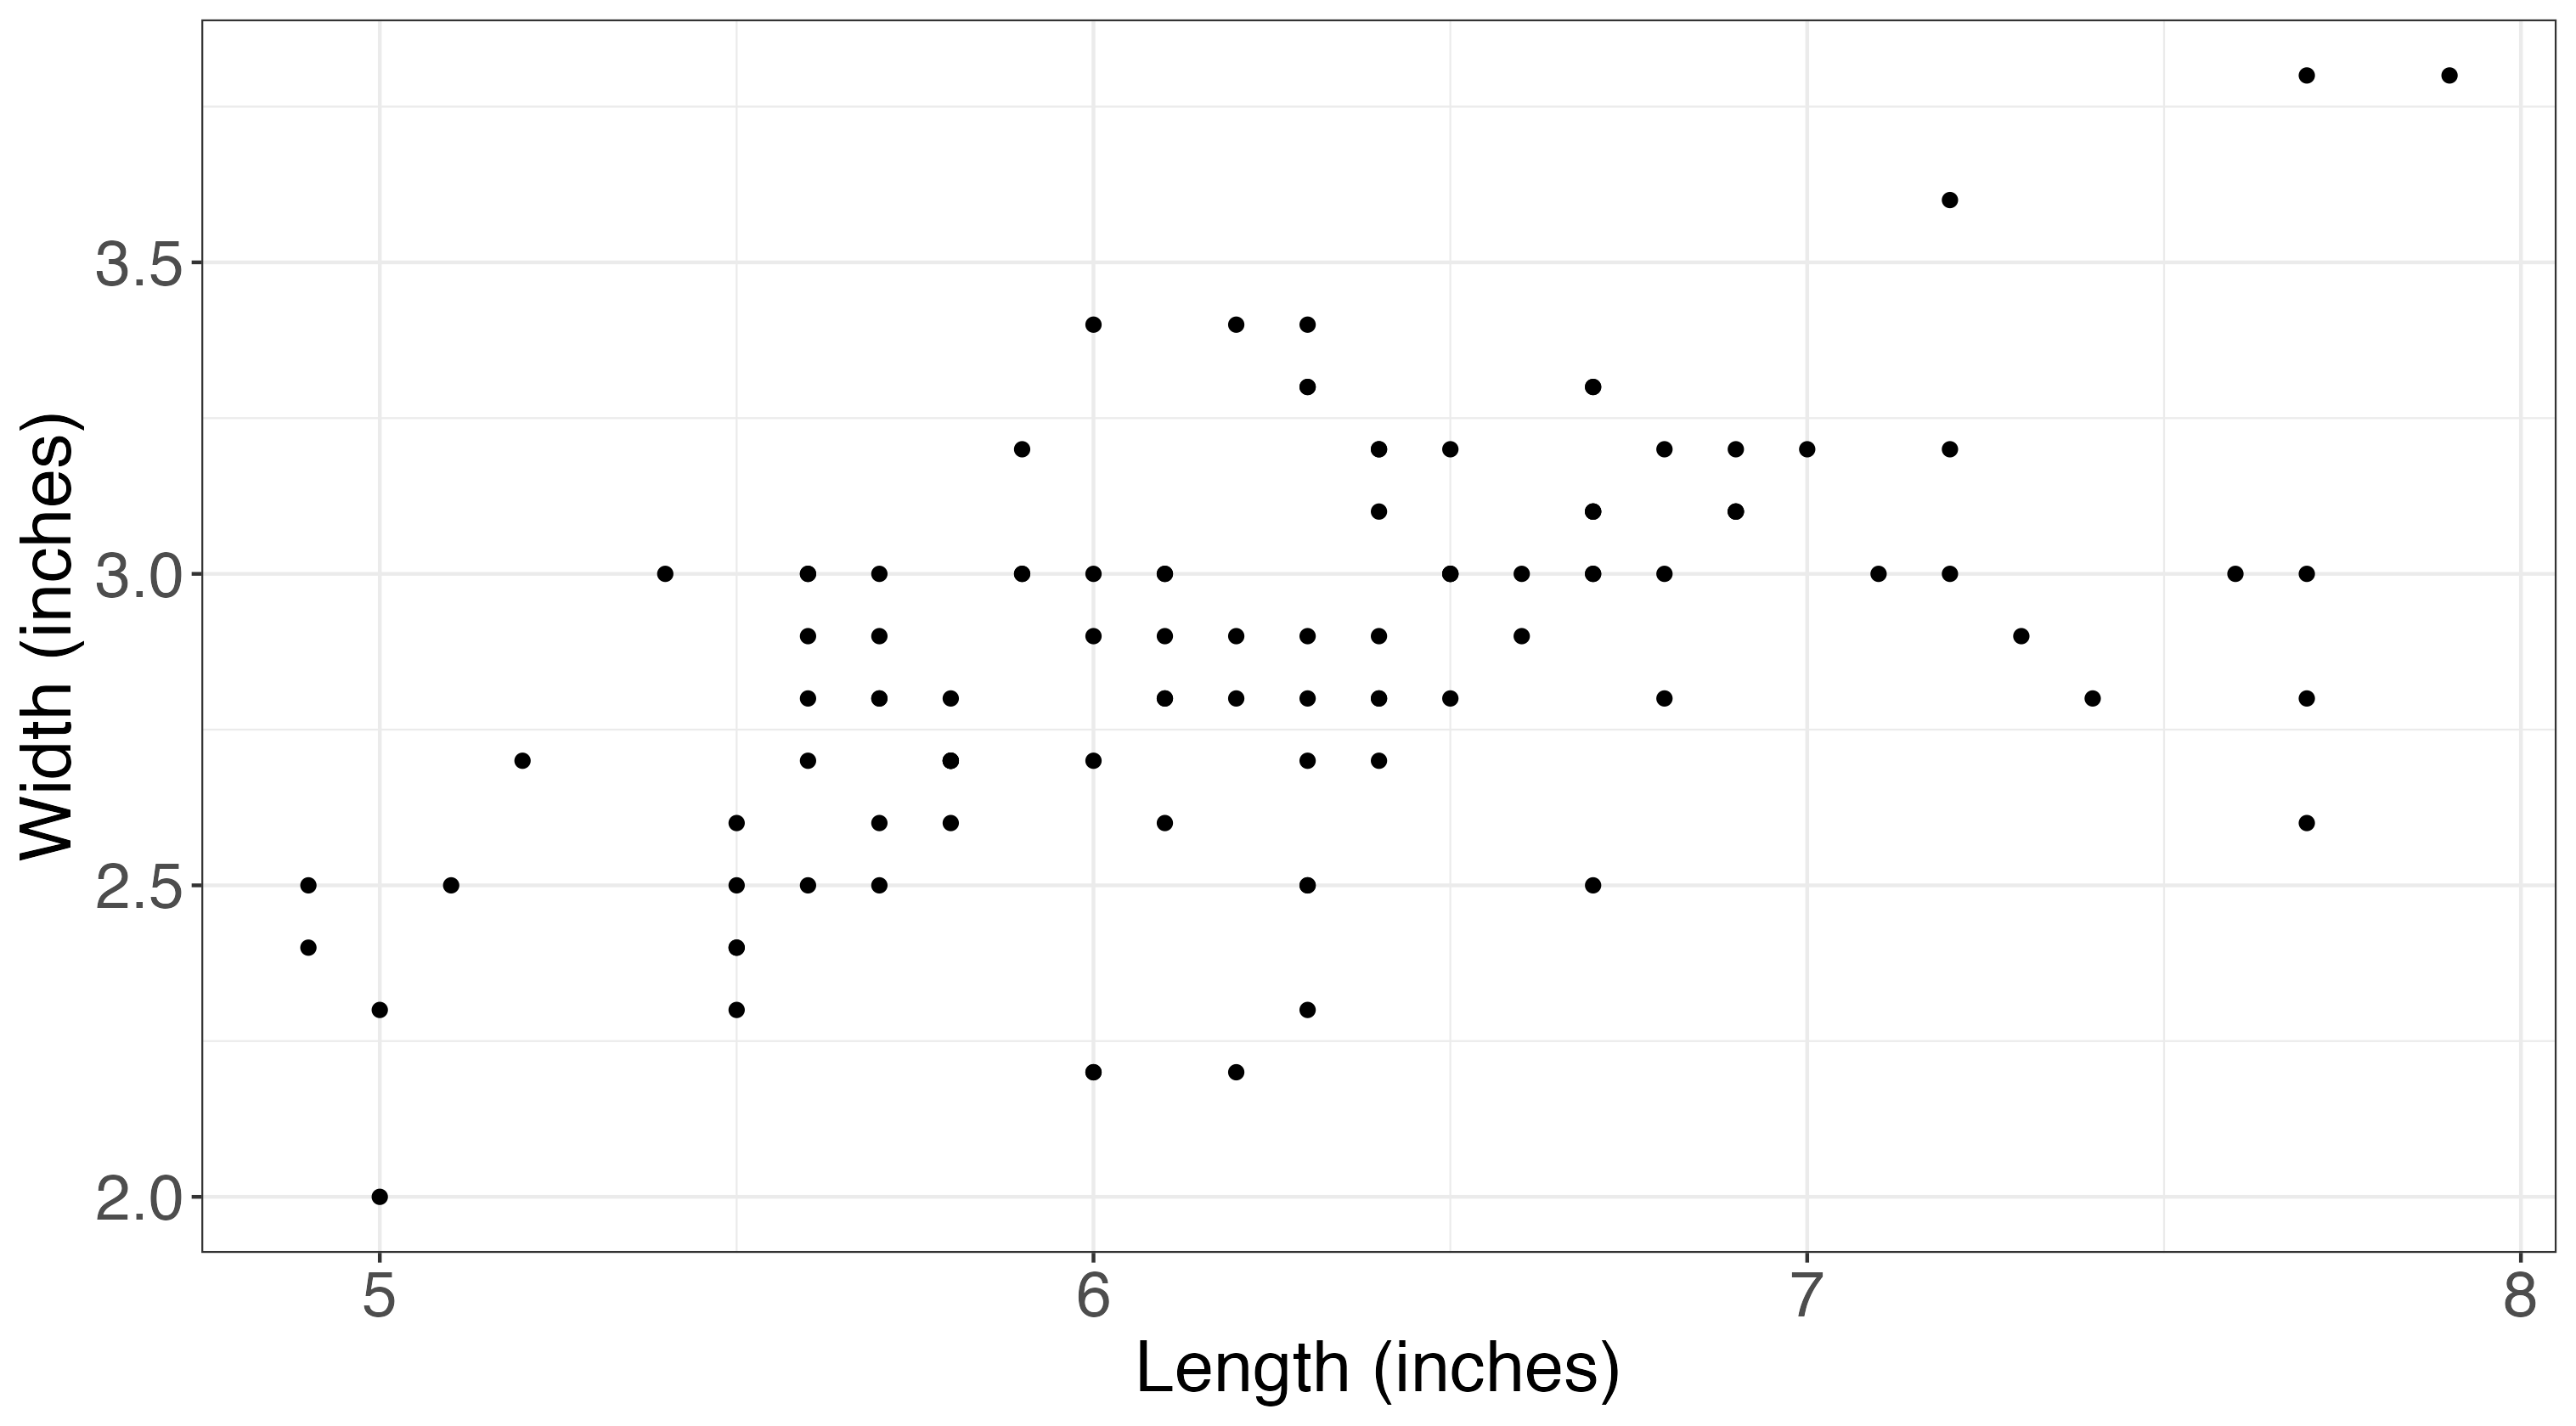
\includegraphics[scale=0.35]{points.png}
\end{figure}

\end{frame}

\begin{frame}{Simple linear regression}
Suppose we want to know how length and width are \textit{linearly} related to each other. To do this, we need to draw a line (\textcolor{red}{$y = a + bx$}) through our data:

\vspace{0.3cm}
\begin{figure}
\centering 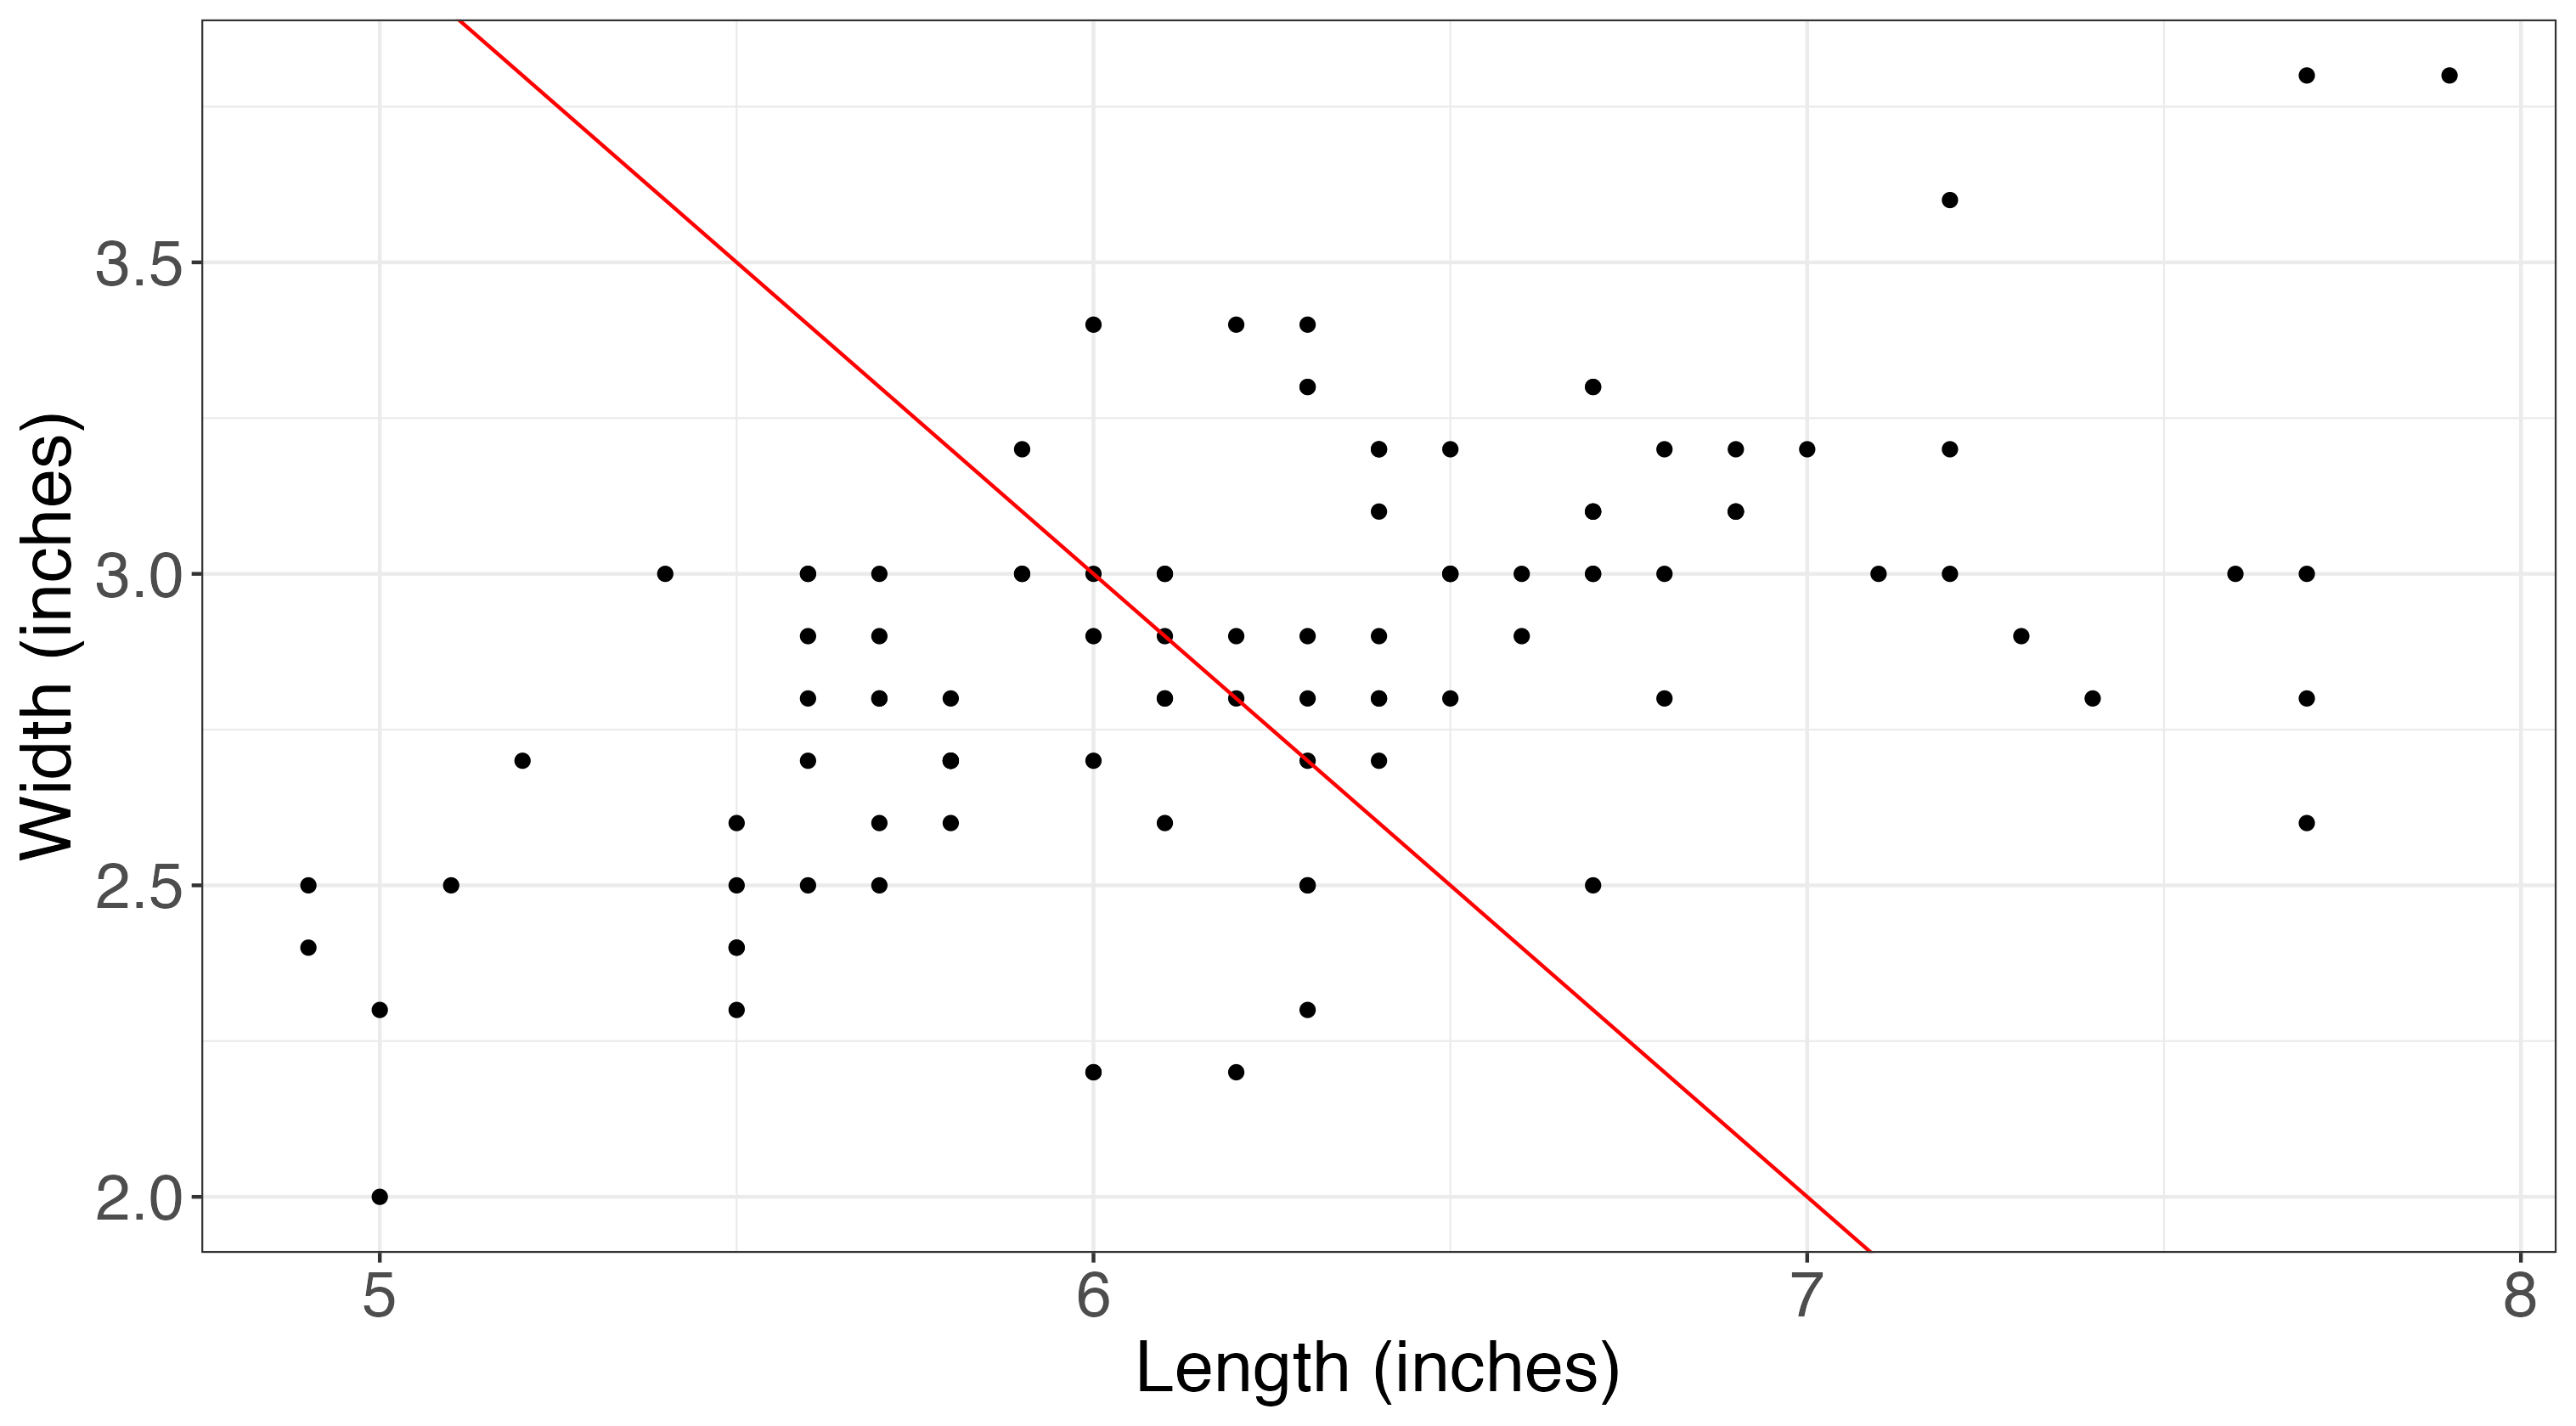
\includegraphics[scale=0.35]{points2.png}
\end{figure}

\end{frame}

\begin{frame}{Simple linear regression}


\begin{figure}
	\centering 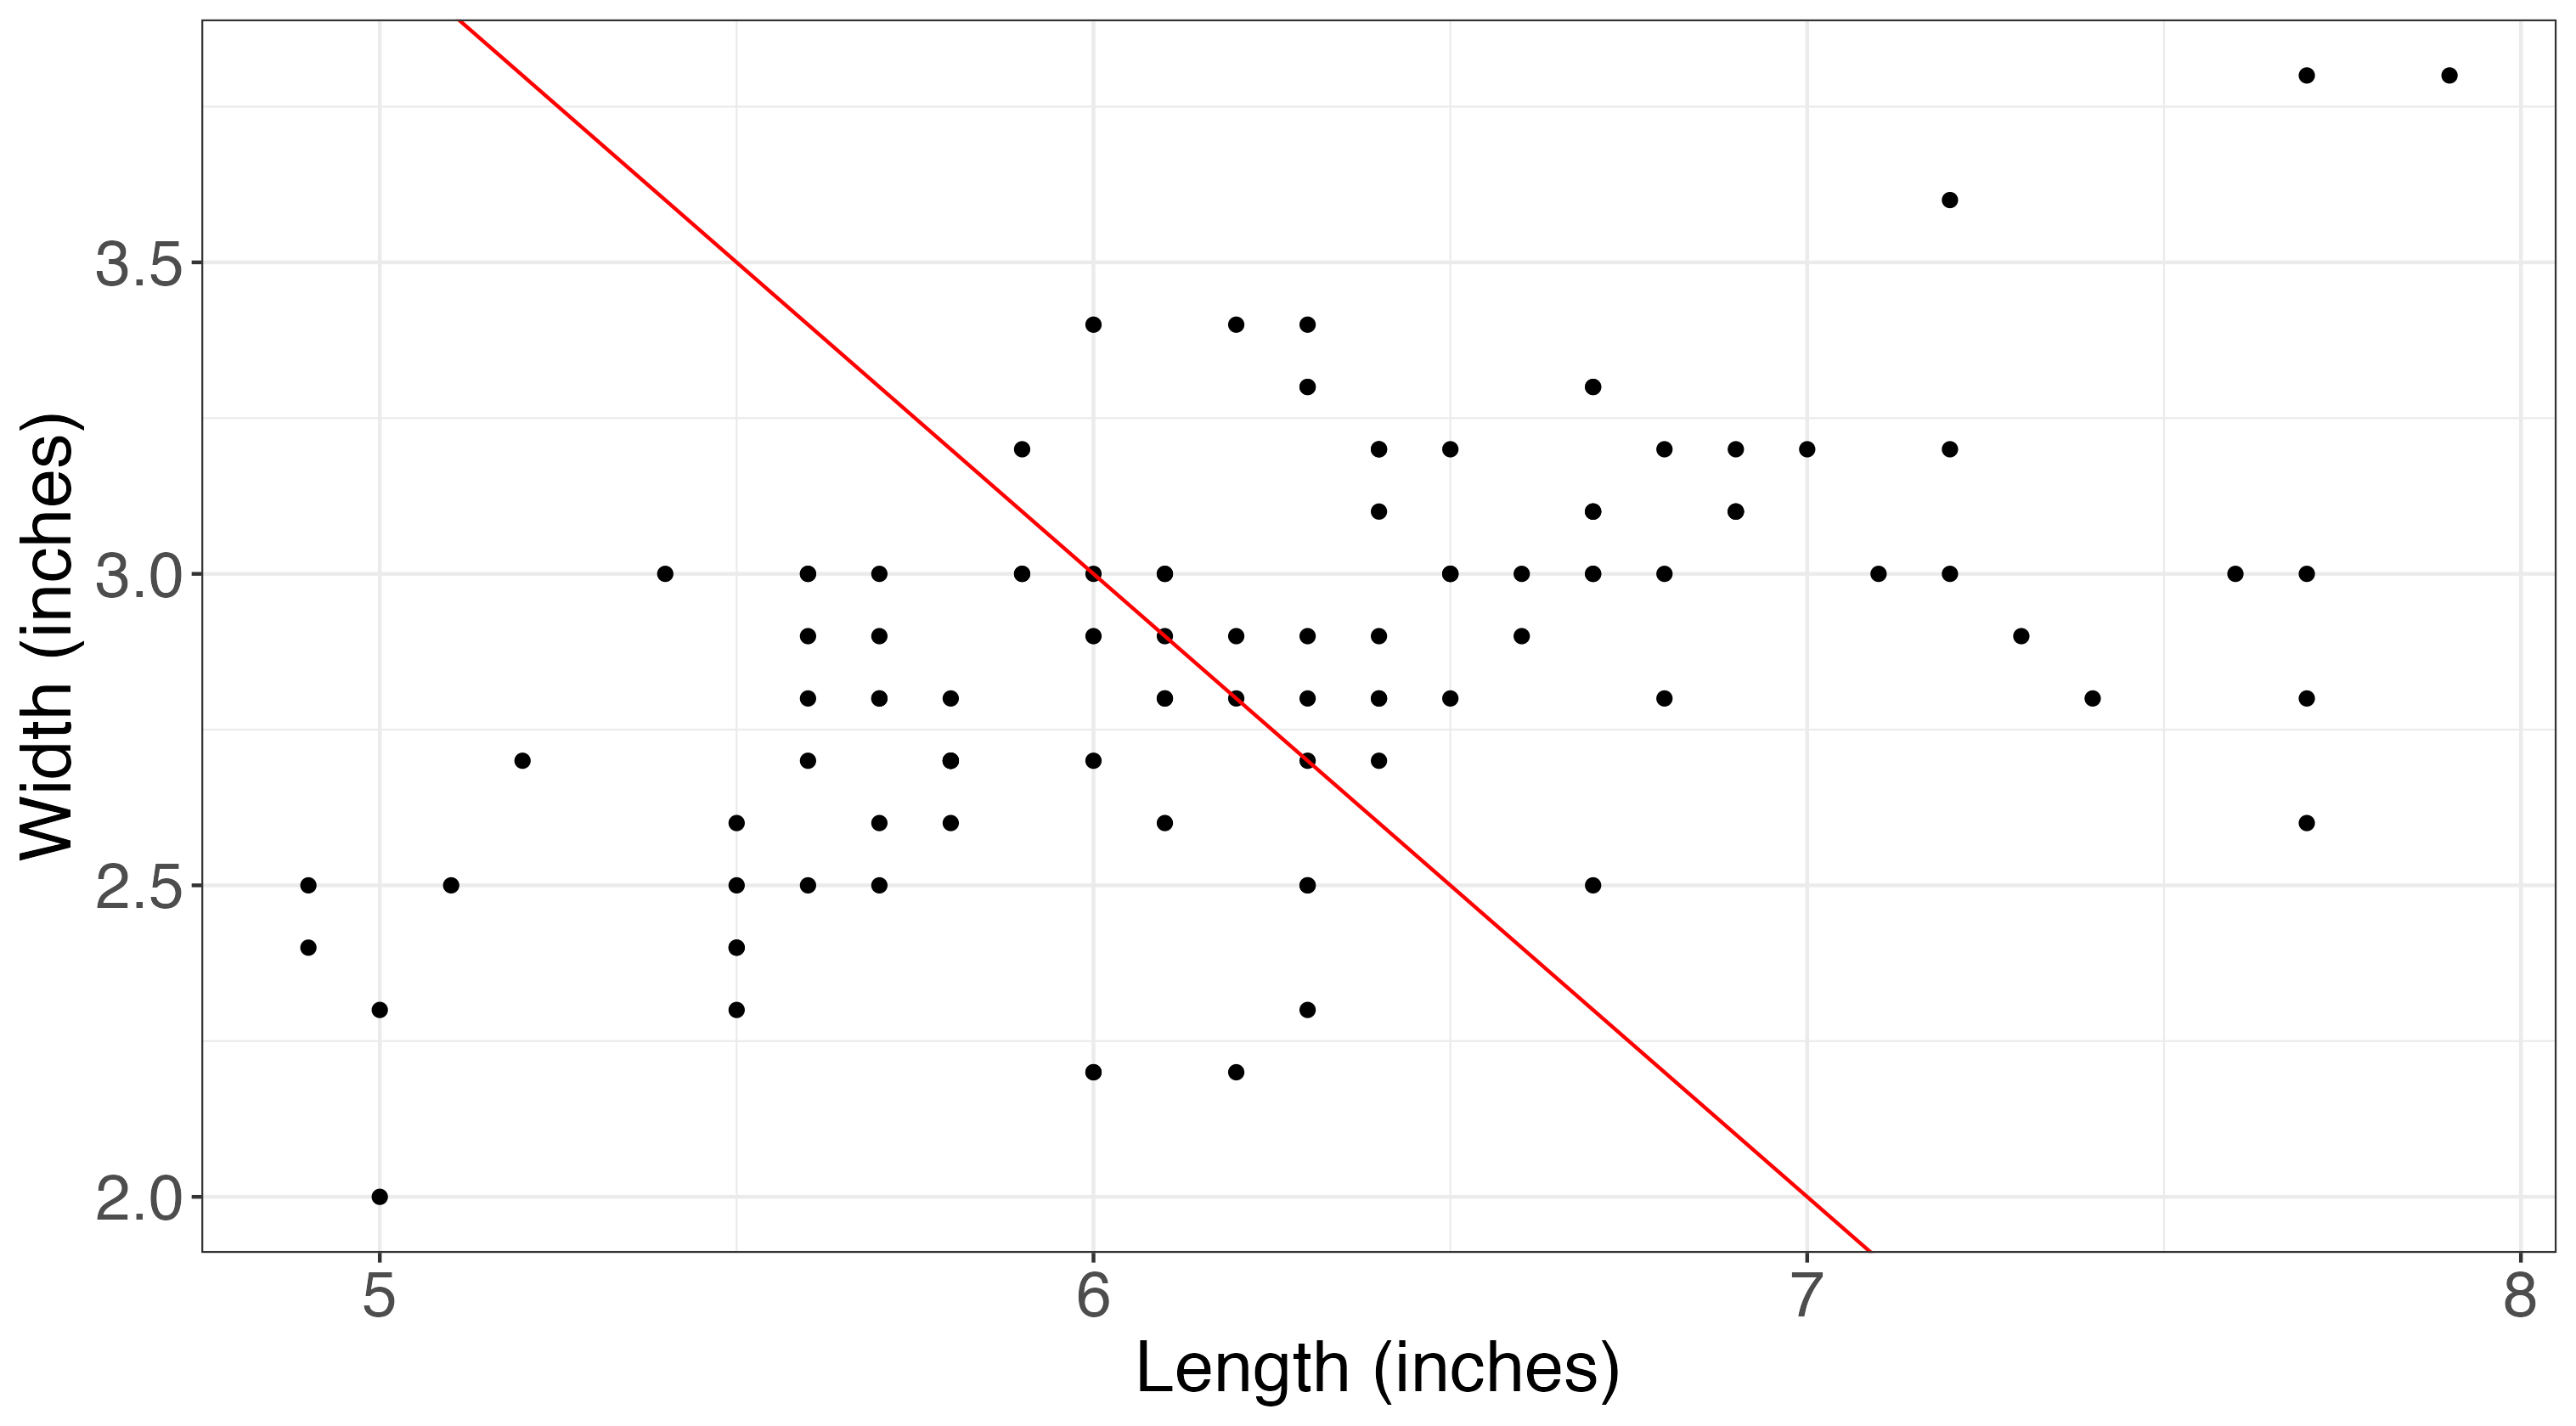
\includegraphics[scale=0.35]{points2.png}
\end{figure}

\vspace{0.3cm}

This line seems bad. Can we articulate \textit{why} it seems bad? Can we articulate why it seems bad \textit{mathematically}?

\end{frame}

\begin{frame}{Simple linear regression}

\begin{figure}
	\centering 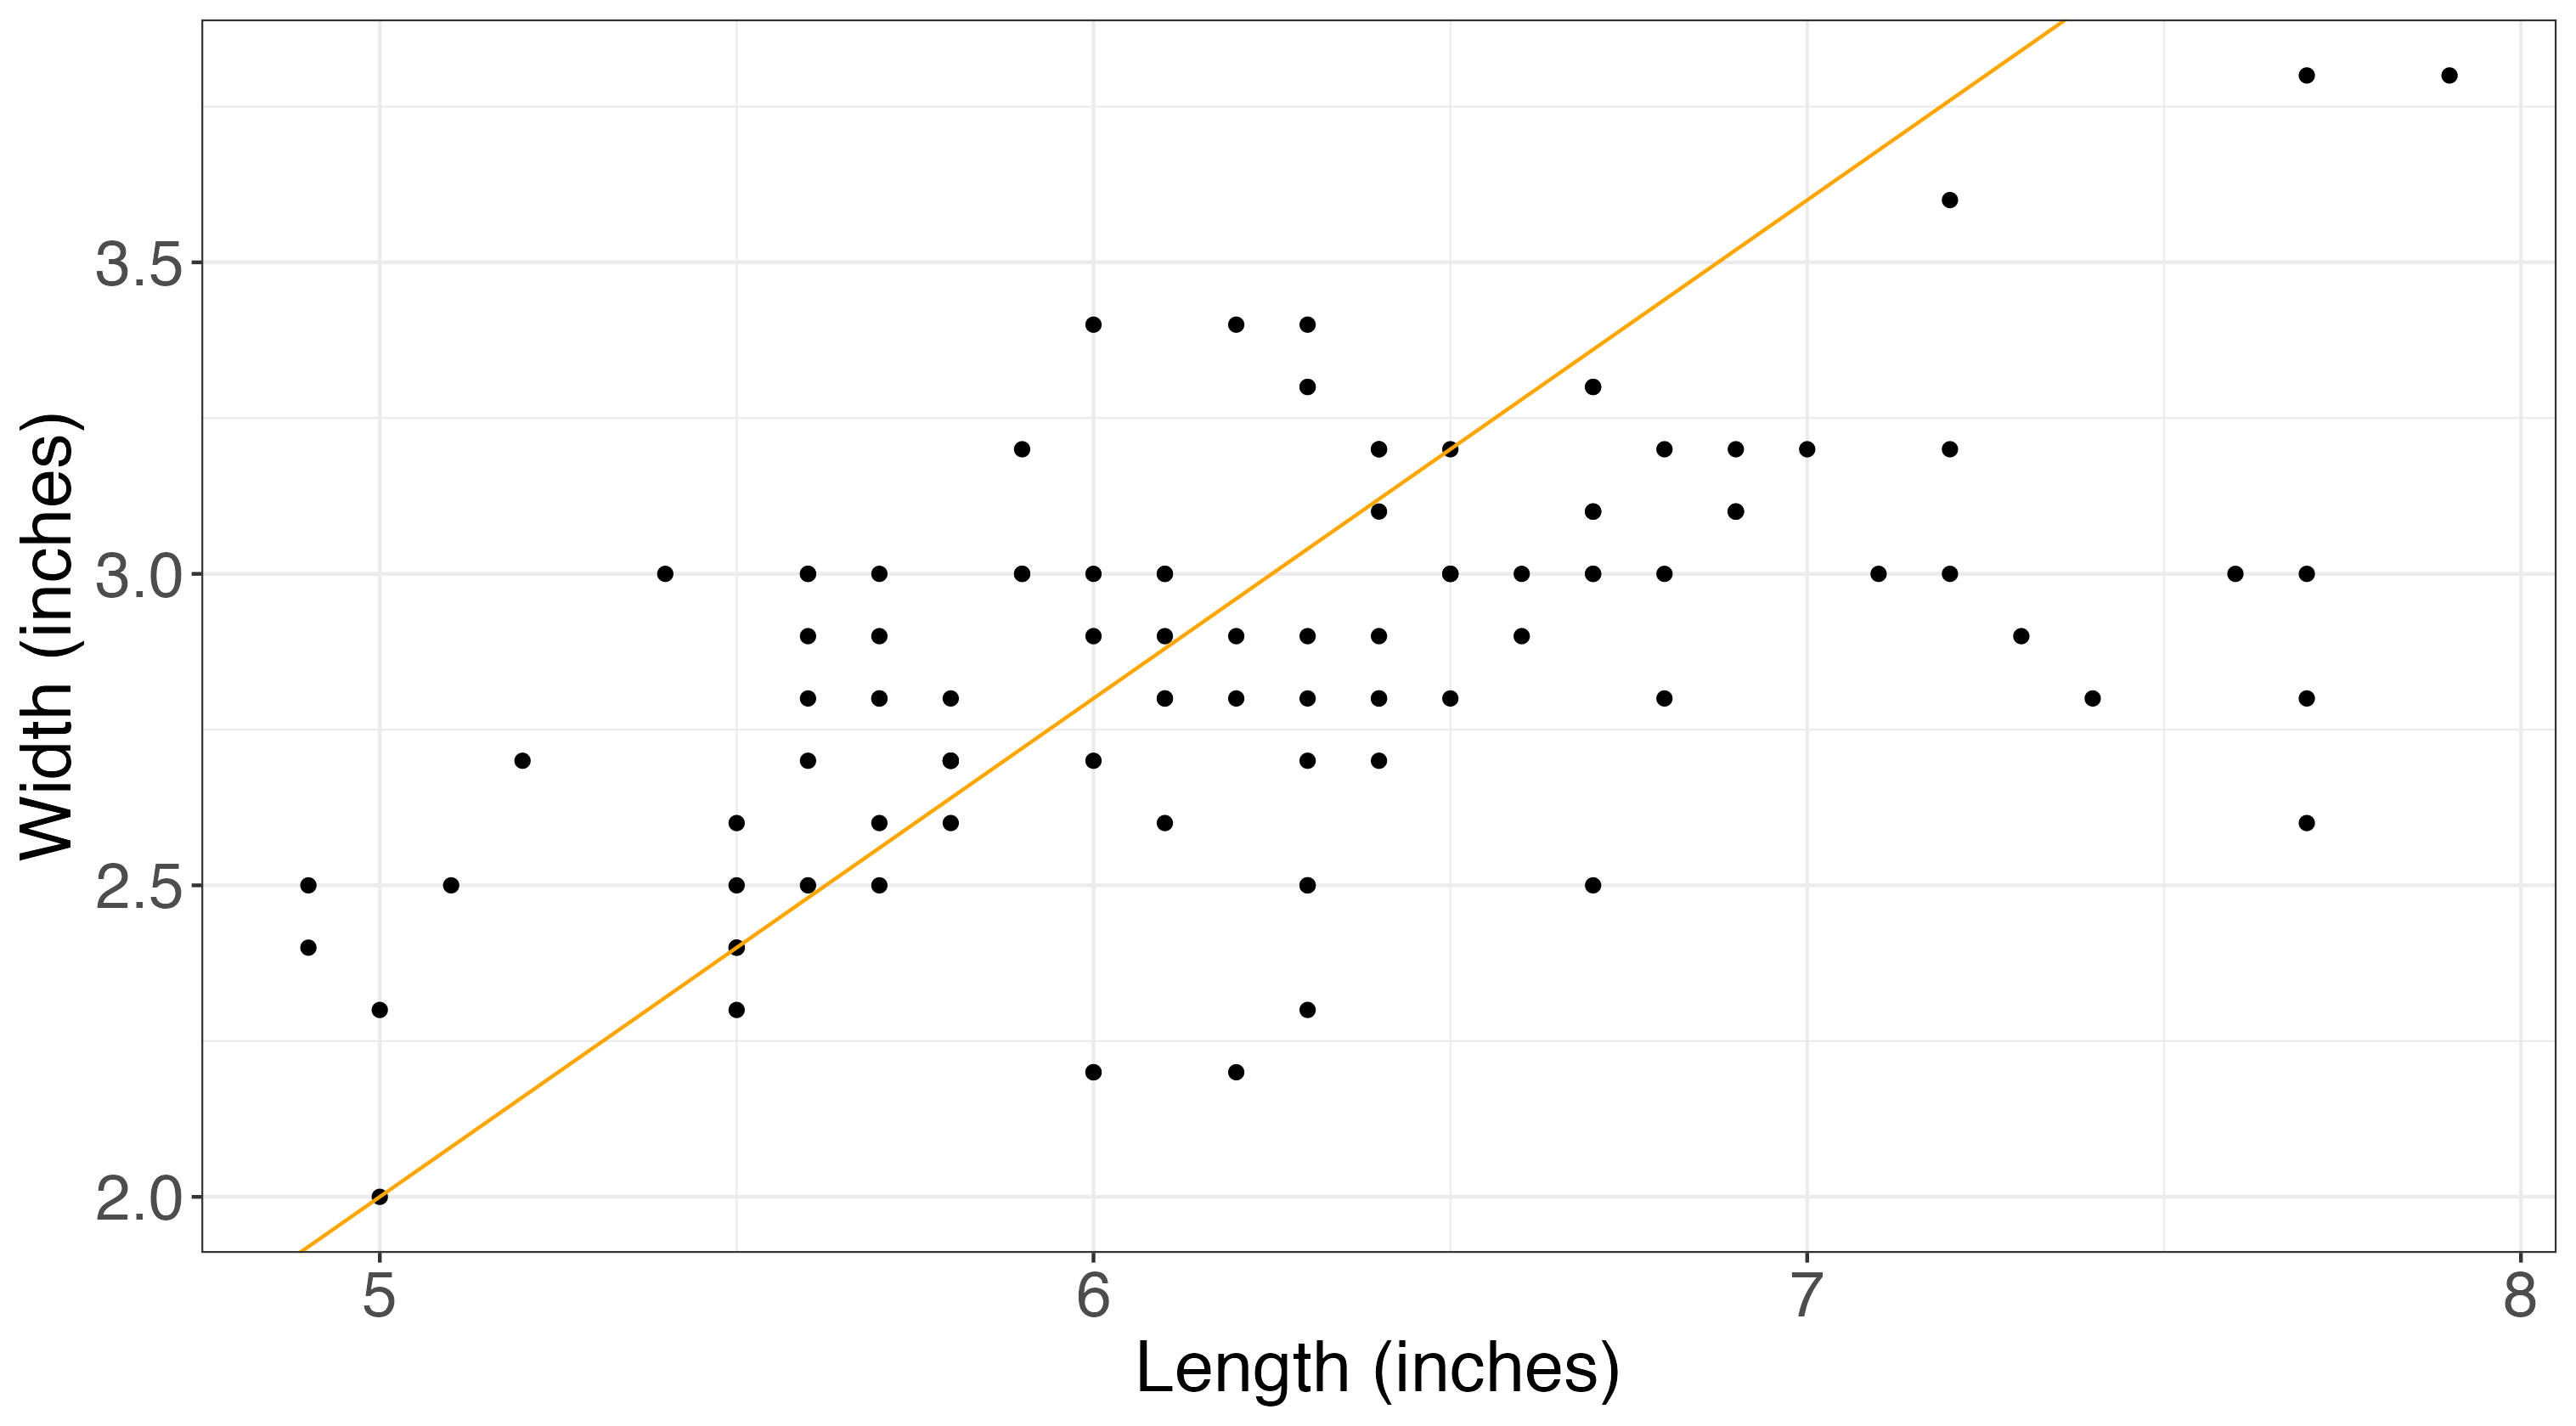
\includegraphics[scale=0.35]{points3.png}
\end{figure}

\vspace{0.3cm}
\small This line seems better! But is it the \textit{best}? And how do we define best?

\end{frame}

\begin{frame}{Simple linear regression}
Simple linear regression is a statistical tool that allows us to estimate the ``best" fitting line through two variables. In general, we use linear regression with \textbf{quantitative} outcomes. Below we show our guesses for the best fitting line and the line estimated from simple linear regression in \textcolor{blue}{blue}:

\begin{figure}
	\centering 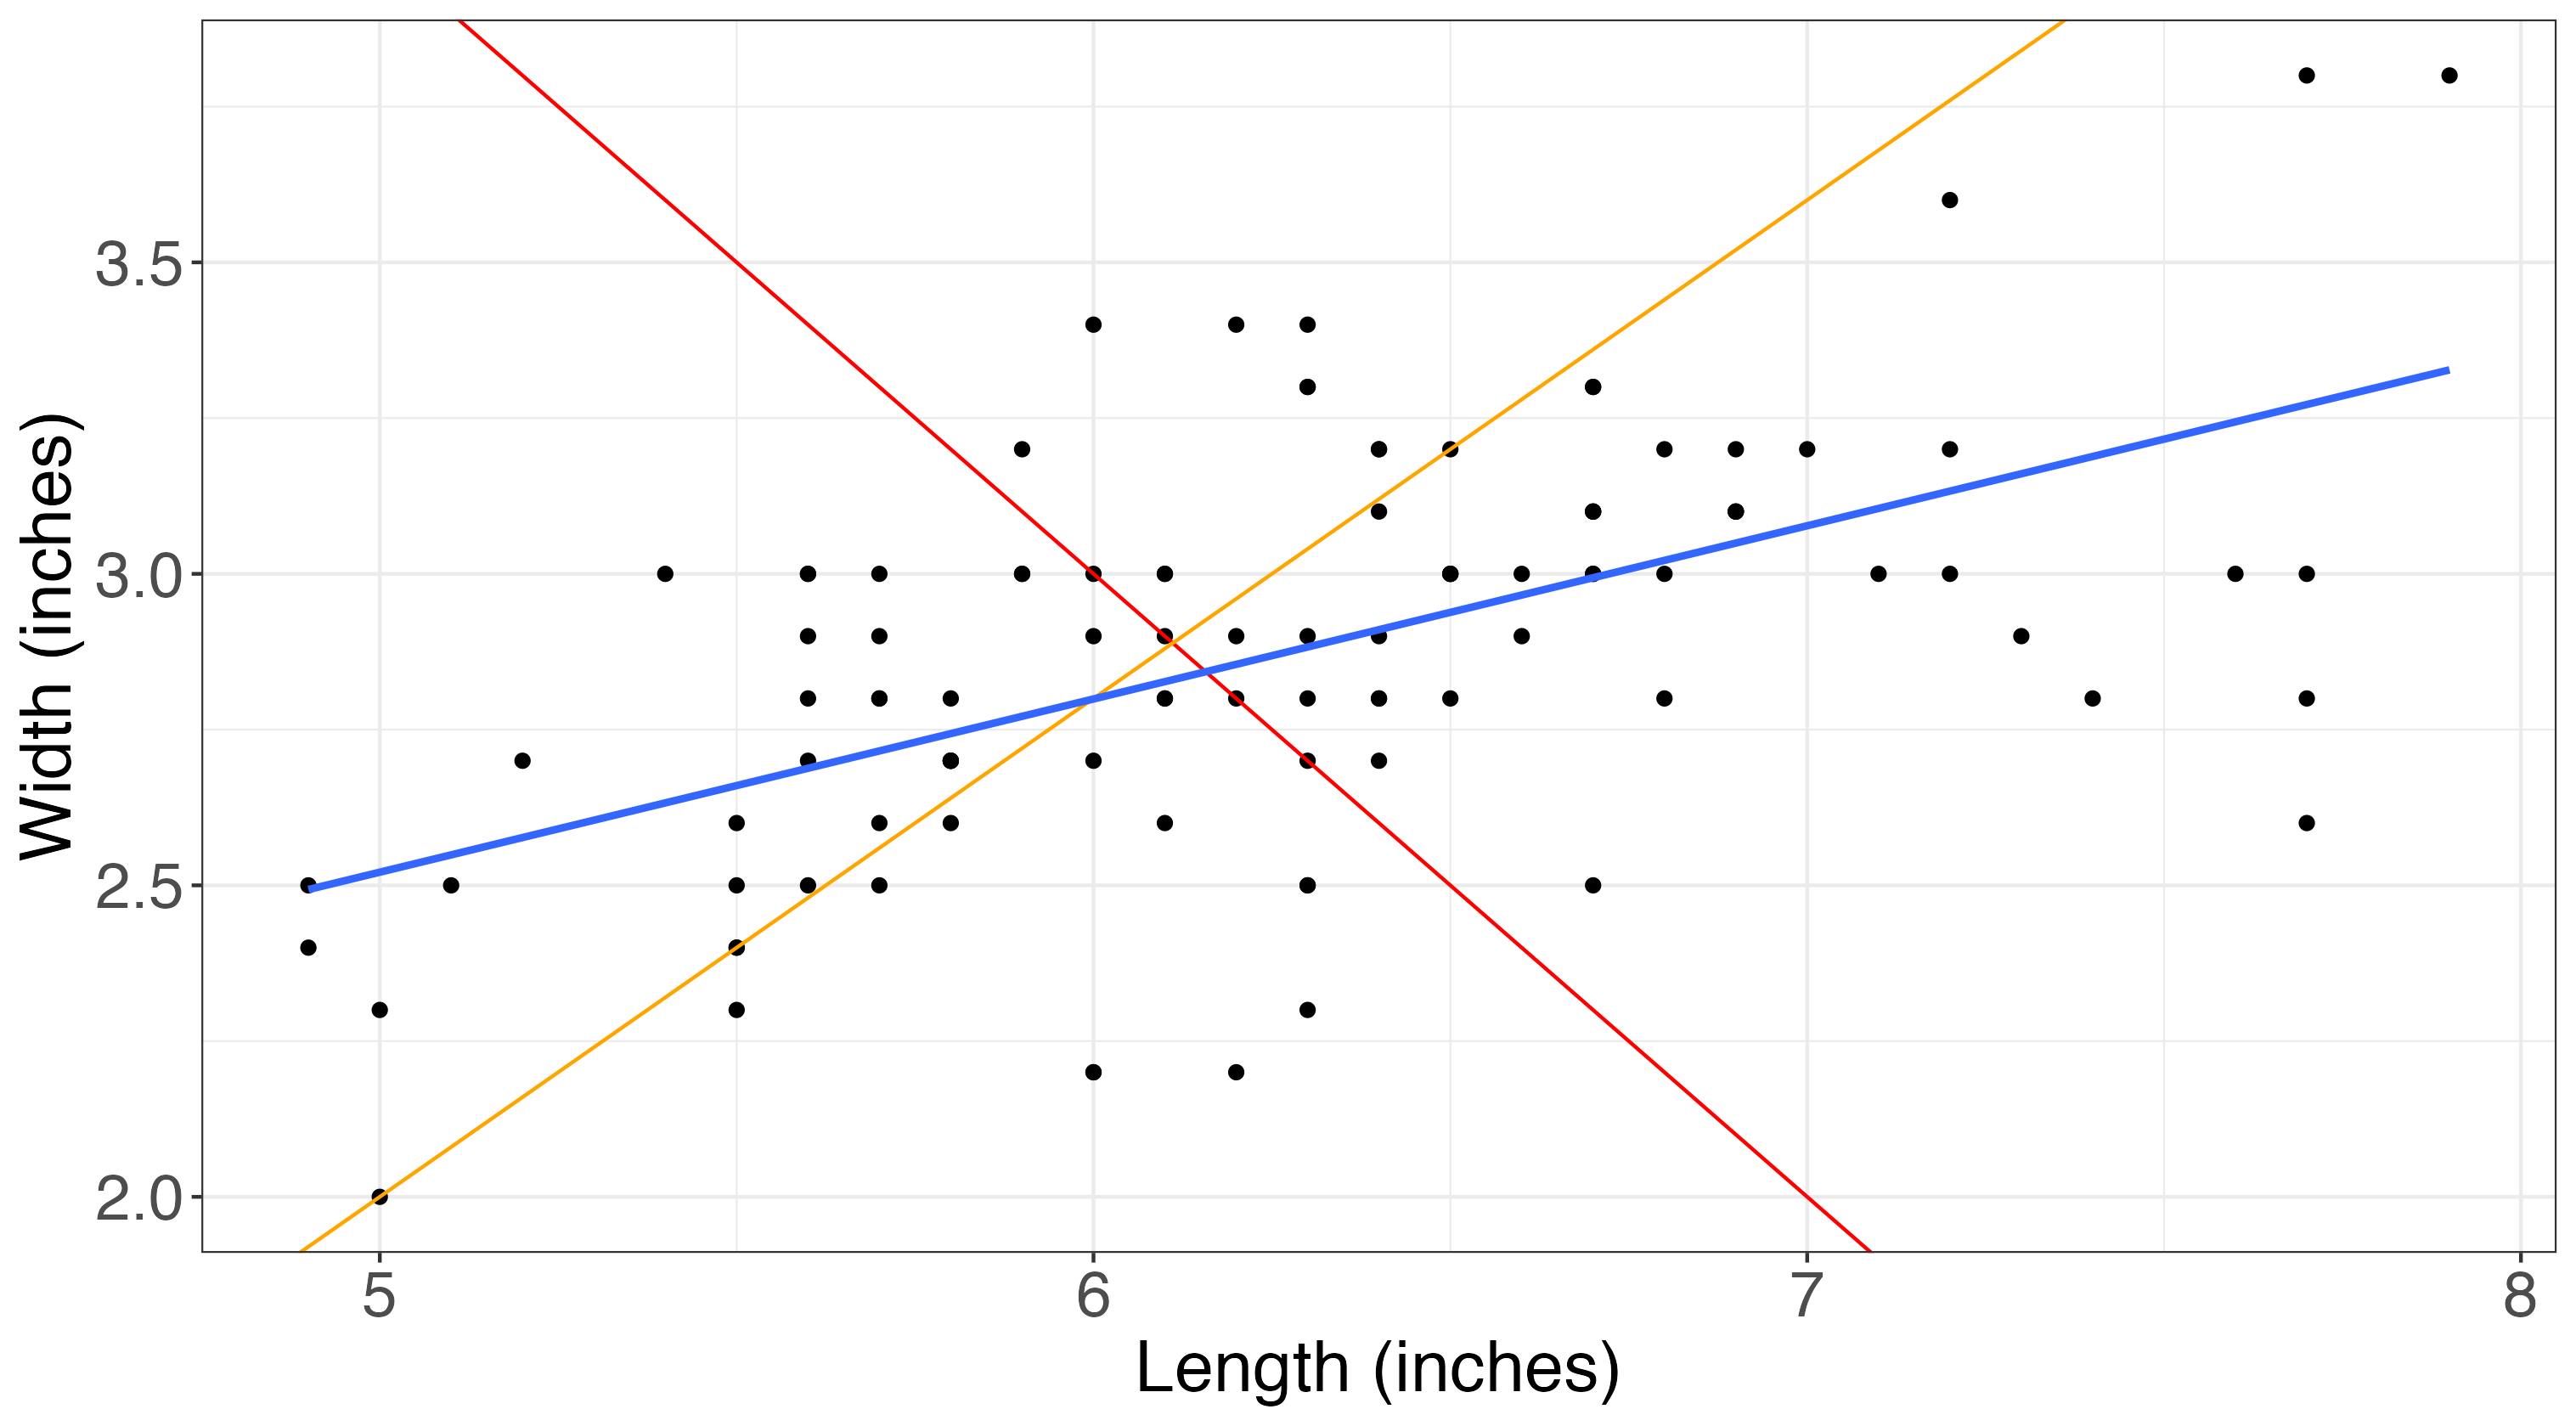
\includegraphics[scale=0.35]{points4.png}
\end{figure}

\end{frame}

\begin{frame}{Simple linear regression}
Lines take the form \textcolor{red}{$y = a + bx$}. When writing regression models we'll use the notation $E[Y \mid X] = \beta_0 + \beta_1 X$. Translating this, we have

\vspace{0.3cm}

\begin{itemize}
	\item $\beta_0$: The intercept of the linear regression line
	\item $\beta_1$: The slope of the linear regression line
	\item $E[Y]$: The average value of $Y$ in the population
	\item $E[Y \mid X]$: The average value of $Y$ in the population, given the predictor $X$
\end{itemize}
\end{frame}

\begin{frame}{Simple linear regression}
Lines take the form \textcolor{red}{$y = a + bx$}. When writing regression models we'll use the notation $E[Y \mid X] = \beta_0 + \beta_1 X$. Translating this, we have

\vspace{0.3cm}

\begin{itemize}
	\item $\beta_0$: The intercept of the linear regression line
	\item $\beta_1$: The slope of the linear regression line
	\item $E[Y]$: The average value of $Y$ in the population
	\item $E[Y \mid X]$: The average value of $Y$ in the population, given the predictor $X$
	\item Examples: $Y$ is birthweight, $X$ is participation in First Steps
	\begin{itemize}
		\item $E[Y] = 3414$ grams (average birthweight in the population)
		\item $E[Y \mid X = 0] = 3424.7$ grams (average birthweight for those not in FS)
		\item $E[Y \mid X = 1] = 3358.5$ grams (average birthweight for those in FS)
	\end{itemize}
\end{itemize}
\end{frame}

\begin{frame}{Simple linear regression: types of predictors}
Our example with heights and widths of leaves had a quantitative outcome \textit{and} a quantitative predictor. 

\vspace{0.3cm}

We can also do simple linear regression with other types of predictors, such as binary or categorical (the illustrative plots just don't look quite as nice). In HW2 you'll get the chance to explore some of this!
\end{frame}

\subsection{Interpretation}


\begin{frame}{Coefficient interpretation}
The coefficients ($\beta_0, \beta_1$) in our simple linear regression model $E[Y \mid X] = \beta_0 + \beta_1 X$ often have useful interpretations.

\vspace{0.3cm} 

How do you interpret $\beta_0$ and $\beta_1$?

\vspace{0.3cm} 

\small (Hint: think about how we interpret $a$ and $b$ in $y = a + bx$)

\normalsize 
\vspace{0.3cm} 

\begin{itemize}
	\item \textcolor{blue}{$\beta_0$} 
	\item \textcolor{blue}{$\beta_1$} 
\end{itemize}

\end{frame}

\begin{frame}{Coefficient interpretation}
The coefficients ($\beta_0, \beta_1$) in our simple linear regression model $E[Y \mid X] = \beta_0 + \beta_1 X$ often have useful interpretations.

\vspace{0.3cm} 

How do you interpret $\beta_0$ and $\beta_1$?

\vspace{0.3cm} 

\small (Hint: think about how we interpret $a$ and $b$ in $y = a + bx$)
\normalsize 
\vspace{0.3cm} 

\begin{itemize}
	\item \textcolor{blue}{$\beta_0$} is the mean value of $Y$ among subjects with $X = 0$
	\item \textcolor{blue}{$\beta_1$} 
\end{itemize}

\end{frame}

\begin{frame}{Coefficient interpretation}
The coefficients ($\beta_0, \beta_1$) in our simple linear regression model $E[Y \mid X] = \beta_0 + \beta_1 X$ often have useful interpretations.

\vspace{0.3cm} 

How do you interpret $\beta_0$ and $\beta_1$?

\vspace{0.3cm} 

\small (Hint: think about how we interpret $a$ and $b$ in $y = a + bx$)

\normalsize 
\vspace{0.3cm} 

\begin{itemize}
	\item \textcolor{blue}{$\beta_0$} is the mean value of $Y$ among subjects with $X = 0$
	\item \textcolor{blue}{$\beta_1$} is the difference in mean value of $Y$ comparing two groups that differ by one unit in $X$
\end{itemize}

\end{frame}

\begin{frame}{Interpreting slopes: mathematical explanation}
For a regression model $E[Y \mid X] = \beta_0 + \beta_1 X$, we noted that the interpretation of the slope $\beta_1$ is the difference in mean value of $Y$ comparing two groups that differ by one unit in $X$. 

\vspace{0.3cm}

Why is this the correct interpretation? Let's do some algebra\dots



\end{frame}

\begin{frame}{Interpreting slopes: mathematical explanation}
For a regression model $E[Y \mid X] = \beta_0 + \beta_1 X$, we noted that the interpretation of the slope $\beta_1$ is the difference in mean value of $Y$ comparing two groups that differ by one unit in $X$. 

\vspace{0.3cm}

Why is this the correct interpretation? Let's do some algebra\dots

\vspace{0.3cm}

\begin{itemize}
	\item $E[Y \mid X = x] = \beta_0 + \beta_1 x$
	\item $E[Y \mid X = (x + 1)] = \beta_0 + \beta_1 (x + 1) = \beta_0 + \beta_1 x + \beta_1$
	\item $E[Y \mid X = (x + 1)] - E[Y \mid X = x] = \beta_1$
\end{itemize}

\end{frame}

\begin{frame}{Practice: interpreting intercepts in context}

Suppose we fit a linear regression model with birthweight (in grams) as our outcome, and age \textit{of birth parent} as our predictor:

\begin{align*}
E[\text{bwt} \mid \text{age}] & = 3161.8 + 8.6 \times \text{age}
\end{align*}

Which of the following is the correct interpretation?

\begin{enumerate}
	\item A child born to a parent of age $0$ will have birthweight equal to 3161.8 grams.
	\item Among all children born to parents of age $0$, the average birthweight is 3161.8 grams.
\end{enumerate}
\end{frame}

\begin{frame}{Practice: interpreting intercepts in context}


\begin{align*}
E[\text{bwt} \mid \text{age}] & = 3161.8 + 8.6 \times \text{age}
\end{align*}

Which of the following is the correct interpretation?

\vspace{0.3cm}

\begin{enumerate}
	\item \sout{A child born to a parent of age $0$ will have birthweight equal to 3161.8 grams.}
	\item \textcolor{blue}{Among all children born to parents of age $0$, the average birthweight is 3161.8 grams.}
\end{enumerate}

\end{frame}

\begin{frame}{Practice: interpreting intercepts in context}


\begin{align*}
E[\text{bwt} \mid \text{age}] & = 3161.8 + 8.6 \times \text{age}
\end{align*}

Which of the following is the correct interpretation?

\vspace{0.3cm}

\begin{enumerate}
	\item[] \textcolor{blue}{Among all children born to parents of age $0$, the average birthweight is 3161.8 grams.}
\end{enumerate}

Questions to consider when interpreting intercepts:

\begin{itemize}
	\item What is the scientific interpretation of ``children born to parents of age 0"? Does our intercept make scientific sense?
	\item Is our intercept within the range of our observed data (i.e. are there parents of age $0$ in our dataset), or would we be \textit{extrapolating} in talking about parents of age $0$?
\end{itemize}

\end{frame}

\begin{frame}{Practice: interpreting slopes in context}
Suppose we fit a linear regression model with birthweight (in grams) as our outcome, and age \textit{of birth parent} as our predictor:

\begin{align*}
E[\text{bwt} \mid \text{age}] & = 3161.8 + 8.6 \times \text{age}
\end{align*}

Which of the following is the correct interpretation?

\begin{enumerate}
	\item For every on year increase in birth parent's age, average birthweight increases by 8.6 grams.
	\item Comparing two groups of birth parents who differ by one year in age, the difference in average child's birthweight will be 8.6 grams, with the higher average birthweight in the older of the two groups.
\end{enumerate}

\end{frame}

\begin{frame}{Practice: interpreting slopes in context}
Suppose we fit a linear regression model with birthweight (in grams) as our outcome, and age \textit{of birth parent} as our predictor:

\begin{align*}
E[\text{bwt} \mid \text{age}] & = 3161.8 + 8.6 \times \text{age}
\end{align*}

Which of the following is the correct interpretation?

\begin{enumerate}
	\item \sout{For every on year increase in birth parent's age, average birthweight increases by 8.6 grams.}
	\item \textcolor{blue}{Comparing two groups of birth parents who differ by one year in age, the difference in average child's birthweight will be 8.6 grams, with the higher average birthweight in the older of the two groups.}
\end{enumerate}


\end{frame}

\begin{frame}{Practice: interpreting slopes in context}
Suppose we fit a linear regression model with birthweight (in grams) as our outcome, and age \textit{of birth parent} as our predictor:

\begin{align*}
E[\text{bwt} \mid \text{age}] & = 3161.8 + 8.6 \times \text{age}
\end{align*}

Which of the following is the correct interpretation?

\begin{enumerate}
	\item \sout{For every on year increase in birth parent's age, average birthweight increases by 8.6 grams.}
	\item \textcolor{blue}{Comparing two groups of birth parents who differ by one year in age, the difference in average child's birthweight will be 8.6 grams, with the higher average birthweight in the older of the two groups.}
\end{enumerate}

Why?
\begin{itemize}
	\item[] This was an observational study! The word ``increases" in the first interpretation implies causality, which we cannot assume in an observational study.
\end{itemize}

\end{frame}

\begin{frame}{Why do we care about the slope?}
In which example(s) is there \textbf{no} association between age and birthweight?

\vspace{0.3cm}

\centering 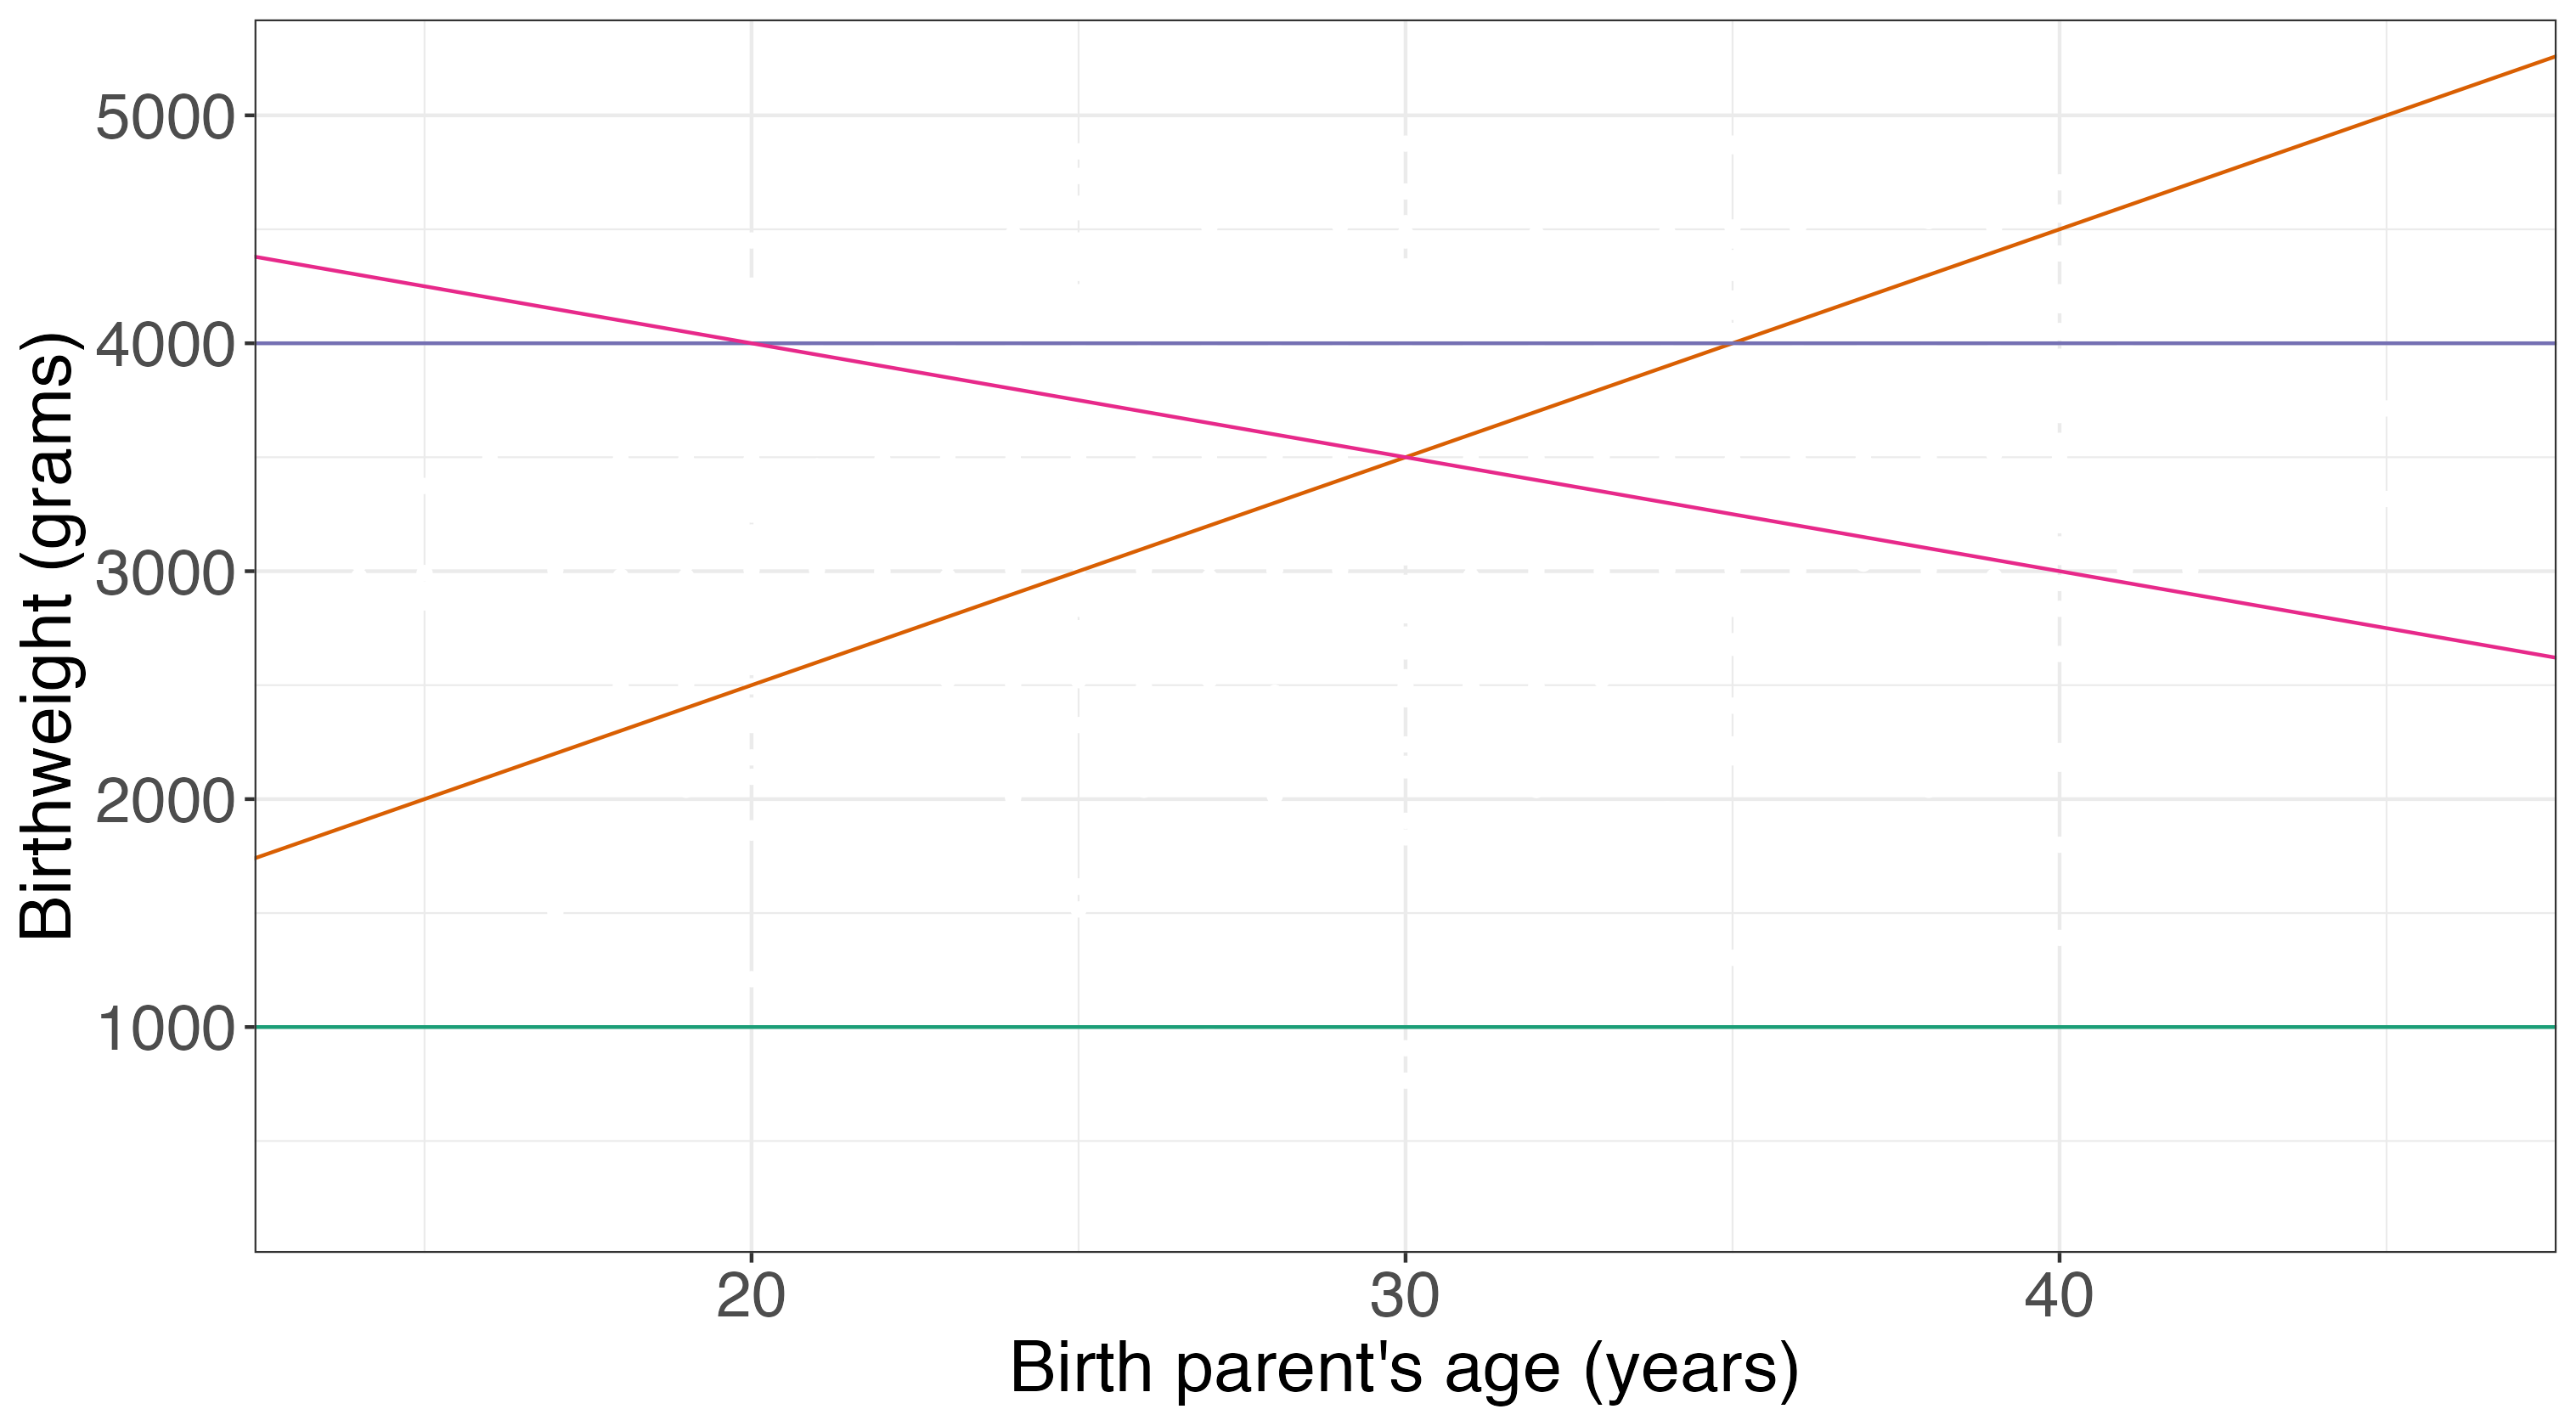
\includegraphics[scale=0.35]{zeroslopes.png}

\end{frame}

\subsection{Assumptions \& diagnostics}

\subsection{Transformations}

\section{Multiple Linear Regression}

\subsection{Adjusting for covariates}

\subsubsection{Confounding (and causal diagrams)}

\subsubsection{Precision variables}

\subsubsection{Effect modification}

\section{Prediction}

\end{document}